\documentclass[11pt, a4paper, oneside]{scrartcl}
\usepackage[textsize=footnotesize,textwidth=3cm]{todonotes}
\usepackage[parfill]{parskip} % Begin paragraphs with an empty line rather than an indent

\newcommand{\Lam}{\Lambda}
\newcommand{\Lamc}{{\bar{\Lambda}}}
\usepackage{amsthm}
\newtheorem{thm}{Theorem}
\newtheorem{theorem}[thm]{Theorem}
\newtheorem{conj}[thm]{Conjecture}
\newtheorem{conjecture}[thm]{Conjecture}
\newtheorem{cor}[thm]{Corollary}
\newtheorem{corollary}[thm]{Corollary}
\newtheorem{lem}[thm]{Lemma}
\newtheorem{lemma}[thm]{Lemma}
\newtheorem{prop}[thm]{Proposition}
\newtheorem{proposition}[thm]{Proposition}

\newtheorem{ax}{Axiom}
\newtheorem{axiom}{Axiom}
\newtheorem{claim}{Claim}
\theoremstyle{definition}
\newtheorem{defn}{Definition}
\newtheorem{definition}{Definition}
\newtheorem{ex}{Example}
\newtheorem{example}{Example}
\theoremstyle{remark}
\newtheorem{notation}{Notation}
\newtheorem{remark}{Remark}
\newtheorem{rem}{Remark}

\PassOptionsToPackage{override}{xcolor} % Beamer option
\usepackage[utf8]{inputenc}
\usepackage{hyperref}
\usepackage{subfig}
\usepackage{amsmath} 
\usepackage{amssymb}
\usepackage{amsfonts,amssymb}
\usepackage{dsfont}
\usepackage[mathscr]{euscript}
\usepackage{enumerate,xspace,threeparttable}
\usepackage{graphicx}
\usepackage{verbatim}
\usepackage{algorithmic}
\usepackage{listings}
\usepackage{wrapfig}
\usepackage{translator}

\providecommand{\ie}{i.e.\ }
\providecommand{\qr}{\eqref}
\renewcommand{\d}{\,d}
\providecommand{\dd}[2]{\dfrac{d#1}{d#2}}
\providecommand{\qtext}[1]{\quad\text{#1 }\quad}

\providecommand{\RR}{\mathbb{R}}
\providecommand{\CC}{\mathbb{C}}
\providecommand{\TT}{\mathbb{T}}
\providecommand{\ZZ}{\mathbb{Z}}
\providecommand{\QQ}{\mathbb{Q}}
\providecommand{\NN}{\mathbb{N}}
\providecommand{\VV}{\mathbb{V}}
\providecommand{\PP}{\mathsf{P}}
\providecommand{\EE}{\mathsf{E}}
\providecommand{\BB}{\mathbb{B}}
\renewcommand{\SS}{\mathbb{S}}

\providecommand{\CF}{\mathscr{F}}
\providecommand{\CB}{\mathscr{B}}
\providecommand{\CA}{\mathscr{A}}
\providecommand{\CR}{\mathscr{R}}
\providecommand{\CH}{\mathscr{H}}
\providecommand{\CM}{\mathscr{M}}
\providecommand{\CT}{\mathscr{T}}

\providecommand{\mfrak}{\mathfrak}
\providecommand{\mscr}{\mathscr}
\providecommand{\mc}{\mathcal}
\providecommand{\mb}{\mathbf}
\providecommand{\bs}{\boldsymbol}
\providecommand{\mbb}{\mathbb}
\providecommand{\ms}{\mathsf}
\providecommand{\vv}[2]{\ensuremath{\overrightarrow{#1#2}}} % vector
\providecommand{\opn}{\operatorname}
\providecommand{\ol}{\overline}
\def\ii#1{^{(#1)}}
\providecommand{\E}{\mathsf{E}}
\renewcommand{\P}{\mathsf{P}}
\renewcommand{\Pr}[1]{\P\left(#1\right)}
\providecommand{\Ex}[1]{\E(#1)}

\providecommand{\Var}{\opn{Var}}
\providecommand{\var}{\opn{var}} 
\providecommand{\Cov}{\opn{Cov}}
\providecommand{\sign}{\opn{sign}}
\providecommand{\diag}{\opn{diag}}

\providecommand{\msf}{\mathsf}
\providecommand{\ett}{\mathsf{1}}

\providecommand{\Ordo}[1]{{O(#1)}} 
\providecommand{\ordo}[1]{{o(#1)}} 
\providecommand{\OrdoOmega}[1]{{\varOmega(#1)}} 
\providecommand{\OrdoTheta}[1]{\ensuremath{\Theta(#1)}} 
\providecommand{\ordoomega}[1]{\ensuremath{\omega(#1)}}

\providecommand{\e}{\epsilon}
\providecommand{\tl}{\tilde}
\providecommand{\g}{\gamma}
\providecommand{\w}{\omega}
\providecommand{\C}{C}
\providecommand{\scp}[2]{\ensuremath{\left\langle#1,#2\right\rangle}}

\providecommand{\bmat}[1]{\begin{bmatrix} #1 \end{bmatrix}}
\providecommand{\T}{^{\!\mathrm{T}}}
\providecommand{\ds}{\displaystyle}

\renewcommand{\L}{\mathscr{L}}

\def\Ex#1{\EE\left[#1\right]}

\def\dom{\opn{dom}}

\def\X{\mscr X}
\def\T{\opn{\msf{T}}}


\def\F{\mscr F}

\def\scp#1#2{\left\langle #1 , #2 \right\rangle}

\usepackage{biblatex}
\addbibresource{main.bib}

\title{Existence for an eigenfunction for the critical phase of the Dyson model}

\author{Anders Johansson, Anders \"Oberg, Mark Pollicott, \\ and Evgeny Verbitskiy}
\date{}
\begin{document}

\maketitle

\def\h{h}


\section{Introduction}\noindent

It is well-known that there exists a continuous and strictly positive
eigenfunction $h$ for any transfer operator defined on a symbolic shift space
with a finite number of symbols such that the potential has summable variations.
Here we prove the existence of an eigenfunction for the important special class
of Dyson potentials close to the critical phase, when the potential does not
satisfy the condition of summable variations.

More precisely, let $T$ be the left shift on the space $X_+=S^{{\mathbb Z}_+}$,
where $S$ is a finite set. Define a transfer operator ${\mathcal L}$ on
continuous functions $f$ by
\begin{equation}\label{trans} {\mathcal L} f(x)= \sum_{y\in T^{-1}x}
  e^{\phi(y)}f(y),
\end{equation}
where $\phi$ is a continuous potential. Since $X_+$ is a compact space, it
follows automatically from the Schauder--Tychonoff theorem that the dual
${\mathcal L}^*$, restricted to the probability measures, has an eigenmeasure
$\nu$: ${\mathcal L}^* \mu=\lambda \nu$, for some $\lambda>0$. The existence of
a continuous eigenfunction $h$ such that ${\mathcal L}h=\lambda h$, $\lambda>0$,
is however not automatic for any continuous potential $\phi$. If one assumes
summable variations of $\phi$,
\begin{equation}\label{sum}
  \sum_{n=1}^\infty \var_n (\phi)<\infty,
\end{equation}
where $\var_n(\phi)=\sup_{x\sim_n y}|\phi(x)-\phi(y)|$ ($x\sim_n y$ means that
$x$ and $y$ coincide in the first $n$ entries), then existence of a continuous
eigenfunction follows from the typical ``cone-argument'' used in {\em e.g.},
Walters \cite{waltersConvergenceRuelleOperator2001}, which to date is the only
known method for providing the existence of an eigenfunction.

If $\mu$ is the equilibrium measure (translation invariant Gibbs measure) for
the continuous potential $\psi:X\to X$, where $X=S^{\mathbb Z}$, then (with
slight abuse of notation) $\mu$ is recovered on $X_+$ as the $g$-measure for the
probability potential
\begin{equation}\label{g}
  g(x)= \frac{h(x) e^{\phi(y)}}{\lambda h(Tx)}.
\end{equation} 
For a transfer operator ${\mathcal L}_g$, defined on continuous functions $f$ by
\begin{equation} {\mathcal L}_g f(x)=\sum_{y\in T^{-1}x} g(y) f(y)
\end{equation}
we have ${\mathcal L}_g^*\mu=\mu$, and also the invariance $\mu\circ
T^{-1}=\mu$.

More precisely, if
$$\theta(x_0, x_1,\ldots)=\beta \sum_{j=1}^\infty \frac{x_j}{j^\alpha},$$
then we may define the two-sided Dyson potential $\psi$ as
$$\psi(x)=\sum_{k=-\infty}^\infty x_k \theta(T^k x).$$ 
A one-sided version can be defined as
$$\phi(x)=\sum_{k=0}^\infty x_k \theta (T^k x).$$
We then have for $\alpha>2$
$$\mu_{|{\mathcal F}_{[0,\infty)}}= h\nu,$$
where $\mu$ is the two-sided translation invariant Gibbs measure (the
equilibrium measure) and where ${\mathcal L}^*\nu=\lambda \nu$, and $h>0$ is a
H\"older continuous eigenfunction. We are interested in the boundary case
$\alpha=2$, when there exists a unique equilibrium measure for $\psi$ for
$\beta<\beta_c$. In this case the summable variations condition is not satisfied
for neither $\psi$ nor $\phi$; we may have multiple eigenmeasures for
${\mathcal L}^*$. In this context we have $\var_n(\phi)=O(\frac{1}{n})$ and it
is not clear if there exists an eigenfunction even in the cases we have a unique
equilibrium measure, such as in the case of the Berbee condition
(\cite{berbeeUniquenessGibbsMeasures1989}) Berbee proved that there exists a
unique equlibrium measure whenever
\begin{equation}\label{berbee}
  \sum_{n=1}^\infty e^{-r_1-r_2-\cdots-r_n}=\infty,    
\end{equation}
where $r_n=\var_n \log \psi$, or if $r_n=\var_n \log \phi$. Berbee's condition
is very robust in the sense that it gives uniqueness for both the two-sided and
one-sided potentials, whereas square summable variations (see
\cite{johanssonSquareSummabilityVariations2003}) only gives a unique
$g$-measure, ${\mathcal L}_g^* \mu=\mu$. Since we have proved in
\cite{johanssonPhaseTransitionsLongrange2017}
that for all $\epsilon>0$ we can find a one-sided potential $\phi$ with
$$\sum_{n=1}^\infty (\var_n \phi)^{1+\epsilon}<\infty$$
such that ${\mathcal L}^* \nu=\lambda \nu$ has multiple solutions $\nu$, it
seems that the existence of a at least a very regular eigenfunction of
${\mathcal L}$ would be in doubt in view of uniqueness of a $g$-measure
corresponding to multiple one-sided Gibbs measures.

Here we prove that if the inverse critical temperature is small enough, close to
the critical phase, then we still have an eigenfunction of ${\mathcal L}$.

\begin{thm}\label{main} Let $\mu$ be the Gibbs equilibrium measure with respect
to the Dyson potential $\phi$ and let $\nu$ be the one-sided Gibbs measure,
i.e., ${\mathcal L}^*\mu=\lambda \mu$. Define
$$h_n(x)=\frac{\mu[x_0,\ldots x_n]}{\nu[x_0,\ldots, x_n},$$
and consider the measurable function $h(x)=\lim_{n\to \infty}h_n(x)$. If
$\beta<\beta_c$, then $h$ is a continuous function on $X_+$, and which is also
an eigenfunction of ${\mathcal L}$.
\end{thm}

We conjecture that there exists a continuous eigenfunction for a potential
$\phi$ that satisfies Berbee's condition \eqref{berbee}.

\subsection{The random cluster model for ferromagnetic Ising spin models}

\def\SI{\{\pm1\}}
\def\SB{\{0,1\}}
\def\b{b}
\def\XI#1{\xi\left(#1\right)}
\def\t{G}

Given a finite graph $(V,E)$ and edge probabilities $p:E\to[0,1]$, $ij\mapsto p_{ij}$, the
Bernoulli graph model $\xi = \xi_p$ is a probability on the set of spanning subgraphs
$\t\subset E$ viewed as functions $\t:E\to\{0,1\}$ such that the probability of each
$\t\in\{0,1\}^E$ is given by
\[ \xi(\t) = p^\t(1-p)^{1-\t} := \prod_{ij}\, p_{ij}^{\t_{ij}}\cdot
  (1-p_{ij})^{1-\t_{ij}}. \]
The expectation of a function $f(\t)$, $\t\in\SI^V$,
with respect to $\xi$ is written $\XI(f(\t))$, i.e.\
\(\XI(f) = \sum_{\t} \xi(\t)\cdot f(\t)\).

An Ising spin vector on $G$ is a vector $x\in\SI^V$ indexed by vertices in $G$.
Consider a potential of the form
\[ H(x) = \beta \sum_{ij\in E} J_{ij} x_i x_j, \] where $J_{ij}\geq 0$ gives the
interaction strength along edge $ij\in E$. The corresponding (ferromagnetic)
Ising model on $G$ is the probability measure $\mu$ where the probability of
$x\in \SI^V$ is given by
\[ \mu(x) = \frac 1{Z} e^{-H(x)}. \]

The \emph{random cluster model} relates the Ising model with a Bernoulli random
graph model as follows: Consider a $\t$ having Bernoulli distribution
$\xi=\xi_p$, where the edge probabilities are
\[ p_{ij} = 1 - e^{-\beta J_{ij}} \quad \text{for $ij\in E$}\] and a uniformly
chosen spin configuration $x\in\SI^V$, i.e.\ where the spins $x_i$ are chosen
from $\SI$ according to a fair coin. We say that $x\in \SI^V$ and $\t\in\SB^E$
are \emph{compatible} if no path in the graph $\t$ connects a spin $x_i=+1$ with
a spin $x_j=-1$, $i\not=j$. We write $\b(\t,x)$ to indicate the event that $\t$
and $x$ are compatible. The joint distribution of $x$ and $\t$ \emph{conditioned}
on the event that they are compatible is what is named the random cluster model
$\rho(x,\t)$. One readily verifies that the marginal distribution of $x$ equals the
Ising model on $\SI^V$ with potential $H$ as above. The marginal distribution of
$\t$ is given by
\[
  \tl\xi(\t) = \frac{2^{\omega(\t)}\xi(\t)}{\xi(2^{\omega(\t)})}
\]
where $\omega(\t)$ denotes the number of connected components in the graph $\t$.

In fact, the probability of a spin configuration $x\in\X_V$ is
proportional to the probability that a $\t\sim\xi(p)$ satisfies $B(\t,x)=1$, which
is proportional to $e^{-H(x)}$. Moreover, the distribution of $\t$ is given by
\[
  \xi'( \t ) = \xi(\t) \frac{2^{\omega(\t)}}{\xi(2^{\omega(\t)})},
\]
where $\omega(\t)$ denotes the number of components (a.k.a.~``clusters'') in $\t$.

\def\cy#1{[x]_{#1}}

For a subset $S\subset V$ of vertices, consider the spin cylinder $\cy S$.
The conditional distribution of $\cy S$, given the graph $\t$, is then clearly
\[ \mu(x_S|\t) = 2^{-\tl\omega_S(\t)} \cdot b(\t, \cy S)\]
where $\tl\omega_S(\t)$ denote the number of clusters in $\t$ that intersects $S$.
Thus
\(\omega(\t)=\ol\omega_S(\t)+\tl\omega_S(\t)\) where $\ol\omega_S(\t)$ gives the
number of clusters in $\t$ that are disjoint with $S$. We obtain that the
marginal distribution of the cylinder $\cy S$ is
\[\mu(\cy S) = \frac{\XI{ 2^{\ol\omega_S(\t)} b(\t,\cy S)}}{\XI{2^{\omega(\t)}}}. \]
If $R\subset S$ then we have
\[\mu(\cy S\mid \cy R) =
  \frac{\XI{2^{\ol\omega_S(\t)} \cdot b(\t,\cy S)}}
  {\XI{2^{\ol\omega_R(\t)} \cdot b(\t,\cy R)}}. \]

\subsection{The one-dimensional Ising-Dyson model}

In the one-dimensional Ising-Dyson model let $V=[-L,L]\subset \ZZ$ and
\[ J_{ij} = \frac \beta{|i-j|^\alpha}.\] We can partition $V$ as $V_- \cup V_+$,
where $V_+=[0,L]$ and $V_-=[-L,-1]$. The random graph $\t^\pm$ is the graph $\t$
induced on $V_\pm$, i.e. $\t_{ij}=1$ only if both ends, $i$ and $j$, are in the
integer interval $V_\pm$. Note that the graphs $\t^+$ and $\t^-$ are independent
under $\xi$. In fact, under the Bernoulli graph model, the graph $\t^+$ is
independent of the graph $\t'=\t\setminus\t^+$.

For $N\ge 0$, let $N$ denote the integer interval $[0,N)$ so that $\cy M = \cy
{[0,M)}$, and $\ol\omega_N = \ol\omega_{[0,N)}$, etc. We also use $\ol N$ to
denote the interval $[N,\infty)$

Let $\mscr L^\pm = \{ C^\pm_1,C^\pm_2, \dots \}$ denote the set of clusters of
the graphs $\t^\pm$ induced on the positive (negative) axis, i.e. the components in the
graphs $\t^\pm$ induced by $\t$ on $V_+$ and $V_-$, respectively. Let $\mscr
R^\pm_N$ be those clusters in $\mscr L^\pm$, respectively, that do not send any
edges to the interval $N=[0,N)$. Thus $\ol\omega_N(\t^\pm)=|\mscr R^\pm_N|$. Let
also $\mscr R''_N$ be the clusters in the graph $\t'=\t\setminus \t^+$ that do
not contain any vertex from $[0,N)$.


\[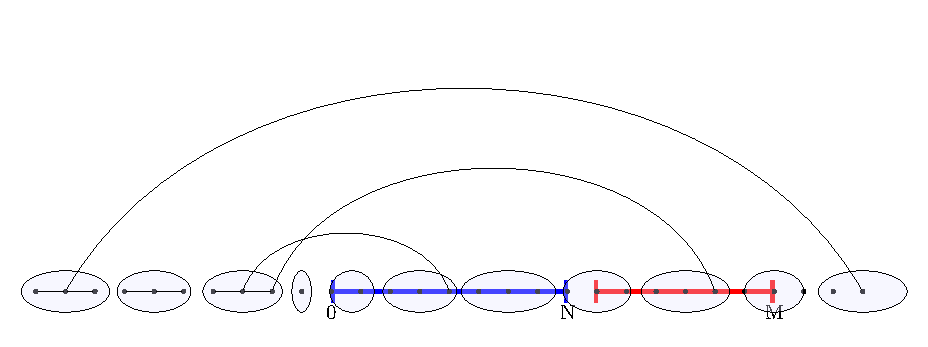
\includegraphics[page=1,width=0.9\textwidth]{fig.pdf}\]

The one-sided Ising model $\nu(x)$ is obtained from the random cluster model with respect
to spins in $V_+$ and the Bernoulli graph model of $\t^+$.
We may write the marginal of the cylinder $\cy N$ for the \emph{one-sided Ising model} as
\[
  \nu(\cy N) =
  \frac{\XI{ 2^{\ol\omega_S(\t^+)} \cdot b(\t^+,\cy N)}}{\XI{2^{\omega(\t^+)}}}
  = \frac{\XI{ 2^{\ol\omega_S(\t^+) + f(\t')} \cdot b(\t^+,\cy N)}}{\XI{2^{\omega(\t^+)+f(\t')}}}.
\]
where $f(\t')$ denotes an arbitrary function of the graph $\t'$.

\def\M{{M}}
\def\N{{N}}



Our aim is to show that for all $x\in\SI^{[0,\infty)}$
\[
  \lim_{M,L\to\infty} \frac{\mu(\cy \M \mid \cy \N)}{\nu(\cy\M \mid \cy\N)} = 1+\ordo N \quad\text{as $N\to\infty$.}
\]

We have
\[
\mu([x]_M|[x]_N)\propto \frac{\XI{ 2^{\ol\omega_M(\t)} \cdot b(\cy M,\t)}}{\XI{ 2^{\ol\omega_N(\t)} \cdot b(\cy N,\t)}},
\]
where we have $\ol\omega_M(\t)=\ol\omega_N(\t)-K_{M,N}(\t)$ and
$b(\cy M),\t)=b(\cy N,\t)\cdot \tilde b_{M,N}(\t)$. Similarly, we have
\[
\nu([x]_M|[x]_N)\propto \frac{\XI{ 2^{\ol\omega_M(\t^+)} \cdot b(\cy M,\t^+)}}{\XI{ 2^{\ol\omega_N(\t^+)} \cdot b(\cy N,\t^+)}},
\]
where $\ol\omega_M(\t^+)=\ol\omega_N(\t^+)-K_{M,N}(\t^+)$ and
$b(\cy M,\t^+)=b(\cy N,\t^+)\cdot \tilde b_{M,N}(x,\t^+)=\tilde b_{M,N}(x,\t)$.

We now prove that $\XI{T<N}=1-o(1)$, as $N\to \infty$.

We define a correction term $C_N(\t',\t^+)$ by the identity $$\ol\omega_N(\t)-\ol\omega_N(\t^+)=f(\t')+C_N(\t',\t^+).$$

We can prove that this correction term is bounded, which follows from the inequality
$$
C_N(\t',\t^+)\leq
E(C_k^2) \cdot \sum _{k=1}^\infty \frac{1}{(N+k)k}<\infty,
$$
where $C_k$ are clusters in $\t[(-\infty, 0])$ ordered after $M(C_k)$,
$M(C_k)\geq k$, and $M(C)=\min \{-i : i\in C \}$.

Conditioned on the event $N>T$, we have that $K_{M,N}(\t^+)=K_{M,N}(\t)$ and that $\tilde b_{M,N}(\t^+)=\tilde b_{M,N}(\t)$.

From the computations above we deduce that
\[
  \frac{\mu(\cy\N)}{\nu(\cy\N)} = \text{const.} \times
  \frac{\XI{2^{\ol\omega_\N(\t)} \cdot b(\t,\cy\N)}}
  {\XI{2^{\ol\omega_\N(\t^+) + f(\t')} \cdot b(\t^+,\cy\N)}}
\]
where the constant is \({\XI{2^{\omega(\t^+)}}}/{\XI{2^{\omega(\t)}}}\).


Then
\begin{equation}
  \ol\omega_N(\t) = \ol\omega_N(\t^+) + \ol\omega_N(\t^-) - X_N(\t') + Z_N(\t)
\end{equation}
where $X_N(\t')$ are the number of edges between clusters in $\mscr R^-_N$ and
$\ol N$. The term $Z_N(\t)$ is a correction term which is not independent of $\t^+$.
However, we have
\[ Z_N(\t) \le Y_N(\t')\]
where $Y_N(\t)$ is the number
\[
  Y_N(\t') = \sum_{C\in\mscr R^-_N} \max\{|E(C,\ol N)|-1,0\}
\]
We claim that $Y_N(\t')$ has distribution bounded by a Poisson variable
$\opn{Po}(\lambda_N)$ where $\lambda_N\to 0$ as $N\to\infty$.


We let
$$A_N^{(m)}= \int 2^{\overline{\omega}([0,N), G^{(m)}}\cdot B([x]_N,G^{(m)}) \; d\xi (G),$$
$$E=\{(i,j): i<0 \wedge j\geq 0\},$$
$$G^{(m)}=G^+ \cup G^- \cup \{(i,j)\in E: |i|+|j|\leq m\},$$
and
$$r^{(m)}=|G^{(m)}\cap E|.$$
We claim that there exist uniform constants $c_1$ and $c_2$ such that
$$0<c_1\frac{A_N^{(m)}}{A_N^{(0)}}<c_2<\infty,$$
where we study $A_N^{(m)}$ such that we have in the extremes
$$A_N^{(0)}=\nu([x]_N)$$
and
$$A_N^{(\infty)}=K\cdot \mu([x]_N).$$

We have
$$X^{(m)}=K\cdot \int 2^{\overline{\omega}_n(G^{(m)})-r^{(m)}(G)}\cdot B([x]_m, G^{(m)})\; d\xi(G),$$
so that
$$X^{(0)}=\nu([x]_n)$$
and
$$\lim_{m \to \infty} X^{(m)}=C\cdot \mu([x]_n).$$
We have furthermore
$$X^{(0)}\geq X^{(1)}\geq \ldots,$$
but we need to prove that the monotone sequence is bounded away from zero.

We have
$$\nu([x]_n)=\frac{ \int 2^{\omega_n(G^+)}\cdot 2^{-\omega_n(G^+)}\cdot B([x]_n, G^+)\; d\xi(G)}{\int 2^{\omega_n(G)} \; d\xi(G)  },$$
where $G^+=G^{(0)}$, and
$$\mu([x]_n)=\frac{ \int 2^{\omega_n(G)}\cdot 2^{-\omega_n(G^)}\cdot B([x]_n, G)\; d\xi(G)}{\int 2^{\omega_n(G)} \; d\xi(G)  }.$$



Let
$$K_m=\min \{|i|: i\in C_m\},$$
where $C_m$ is the $m$th cluster. Note that $K_m\geq m$.

We will prove that if $A_n$ is the event that we send one edge from the negative to the positive side (beyond 0), as well as one edge from the negative side beyond $n$, then $P(A_n)\to 0$.

The probability of an edge from cluster $C_i$ (e.g.\ on the negative side) to cluster $C_j$ (e.g.\ on the positive side) is
$$1-e^{-\sum_{C_i} \frac{\beta}{|i-j|^{\alpha}}}.$$

We have
$$\sum_{-k\in C}\frac{\beta}{n+k}\leq |C|\cdot \frac{1}{K_C}\cdot \beta.$$
Hence the probability of valence $\geq 2$ is
$$\leq  |C|^2\cdot \frac{1}{K_C^2}\cdot \beta^2.$$
Since then
$$\sum \frac{C_m^2}{K_m^2}<\infty,$$
we have by the Borel--Cantelli lemma only finitely many clusters with valence
$\geq 2$.


\section{Proof of the main results}\noindent

\begin{lem}
  There exists a continuous eigenfunction $h$ of ${\mathcal L}$, if
$$\frac{\mu[x_0,\ldots x_N, \ldots, x_n]}{\nu[x_0,\ldots, x_N, \ldots, x_n]}=(1+o(1)) \frac{\mu[x_0,\ldots, x_N]}{\nu[x_0, \ldots, x_N]},$$
as $N\to \infty$.
\end{lem}
\begin{proof}
  Let $\lambda=1$. By the assumption, the measure $\mu= \h \nu$ is translation
  invariant, i.e., $\mu\circ T^{-1}=\mu$. Hence we have $(h\nu)\circ
  T^{-1}=h\nu$ and it suffices to show that $(h\nu)\circ T^{-1}=({\mathcal
    L}h)\nu$.

  Let $A$ be any Borel subset of $X_+$. Then
  $$(h\nu)\circ T^{-1} (A)=\int_A \sum_{y: Ty=x} h(y)e^{\phi(y)}\; d\nu(x)=\int_A h(x)\; d\nu(x).$$
\end{proof}

\begin{lem}
  If $$\frac{\mu[x_0,\ldots x_N, \ldots, x_n]}{\nu[x_0,\ldots, x_N, \ldots, x_n]}=e^{\xi}\; \; \frac{\mu[x_0,\ldots, x_N]}{\nu[x_0, \ldots, x_N]},$$
  then $|\xi|=O(P(A_N))$, where $A_N$ is the event that there exists a cluster
  $C\subset [(-\infty, 0]$ with two edges that goes from $C$ into $[N,\infty)$.
\end{lem}
\begin{proof}
  For the random cluster model, we have that
  \[
    \mu[x_0,\ldots, x_N]\propto P((t_{ij} \sim [x_0, \ldots, x_N]),
  \]
  where $\sim$ means that the graph $t_{ij}$ is compatible with the cylinder
  $[x_0,\ldots, x_N]$.

  We will study conditional probabilities $P(B_M|B_N)$, where $B_M$ means
  $t_{ij}\sim [x_0,\ldots, x_M]$.

  We have
  \[
    e^{\xi}=
    \frac{K(x_0,\ldots, x_N)P(B_M|B_N)}{\tl K(x_0,\ldots, x_N)P(\tilde B_M|\tilde B_N)}.
  \]

  We make a coupling with the one-sided system $\tilde t=t[0,\infty)$ and use
  the corresponding events $\tilde B_M: \tilde t \sim [x_0,\ldots, x_M]$. Notice
  that $B_M\subset \tilde B_M$.

  We have
  \[
    \frac{P(B_M|B_N)}{P(\tilde B_M| \tilde B_N)} = \frac{P(B_M|\tilde B_M, B_N) \P(\tilde B_M|B_N)} {P(\tilde B_M|\tilde B_N)} = \P(B_M|\tilde B_M, B_N)=e^{o(1)},
  \]
  as $N\to \infty$, independently of $M$.
\end{proof}

\begin{lem}
$$\lim_{N\to \infty} P(A_N)=0.$$
\end{lem}

\begin{proof}
  Let $M(C)=\inf \{i\in C \}$ and let $S=P(A_N |t[(-\infty, 0]])$.

  We have
$$P(A_N|t[(-\infty, 0]])\leq K \sum_{k=1}^\infty \frac{C_k}{N+M(C_k)}.$$
The conclusion follows from $E(S)<\infty$.

Let $X(C)$ be the number of clusters $C$ that have edges between $C$ and
$[N,\infty)$. By assuming that $X(C)\sim P_0(\lambda)$, we can make the estimate
$$P(X(C)\geq 2)\leq c\cdot \lambda^2 \leq c\cdot \frac{|C|^2}{(N+M)^2}\cdot \beta^2,$$
where $c=\sum_{k=2}^\infty e^{-\lambda} \frac{\lambda^k}{k!}$.

We have
$$E(S) \leq K \sum_{k=1}^\infty \frac{E(C_k^2)}{(N+k E(C_k))^2},$$
where $C_k$ are clusters in $t[(-\infty, 0])$ ordered after $M(C_k)$,
$M(C_k)\geq k$. We can make an estimate
$$E(S)\leq E(C_k^2)\sum _{k=1}^\infty \frac{1}{(N+k)^2},$$
which proves the lemma, since $E(C_k^2)<\infty$ by
\cite{aizenmanUniquenessInfiniteCluster1987}.

\end{proof}





\section{Nytt}
\hrule 

Let $G=(G^+, G^- , E)$, $\gamma=(G^+,G^-)$.

We have
$$d\tl\nu(G)=2^{\omega(G^+)+\omega(G^-)-|E|-\rho_{|E|}}\; d\xi(G),$$
where $\xi$ is the Bernoulli measure, and $E$ is the set of edges from the minus side to the plus side. The term $\rho_{|E|}$ normalises, i.e.\
\[
\rho_{|E|} = 
\log \int 2^{\omega(G^+)+\omega(G^-)-|E|}\; d\xi(G).
\]
Notice that
$\omega(G^-)-|E|$ is independent of $G^+$, and so we have $\nu\circ (G^+)^{-1}=\nu(G^+)$.

We have 
$$d\mu(G)=2^{q(G)-\rho_q}\; d\nu(G),$$
where $\rho_q$ just normalises $\mu$ and where $q(G)$ is the co-rank in the set $E$, i.e., 
$$
q(G)=\max \{|E|-|T\cap E|\mid \text{$T$ spanning tree of $G$} \}.
$$
Consider the graph $G_{ij}\subset E$ where for $i,j>0$
$$ G_{ij} =  \gamma \cup 
\{ kl\in E \mid k < i \text{ or } k=i \text{ and } 0>l>-j \}.
$$
We also denote $G_m = \lim_{j\to-\infty} G_{mj}$. 
We can define $q(G)$ as the number of edges between $i$ and $-j<0$ that connects vertices ``already'' connected in $G_{ij}$. 
It is also clear that $q$ is less than or equal to the number of 
cluster in $G^-$ incident with more than one edge of $E$.


We claim that,
$$
P(q|\gamma)\approx \operatorname{Po}(\lambda(\gamma))
$$
where $\lambda(\gamma) = \mathsf E(q|\gamma)$. We have 
\[
\lambda(\gamma) = \sum_{i=0}^{\infty} \sum_{j=1}^{\infty} (1-e^{-\frac{\beta}{(i+j)^2}}) 
\mathsf P(i\sim_{G_{ij}} -j\mid \gamma).
\]
where $a\sim_H b$ states that there is a path between $a$ and $b$ in the graph $H$. 

Since $G_{ij}$ is stochastically dominated by $G$ we obtain that 
\[
\P(i \sim_{G_{ij}} -j) \le \P(i \sim_G j) = \tau(i+j),
\]
where $\tau(n)$ is the usual two-point correlation function 
\[
\tau(n) = \mathsf P(0\sim_G n).  
\]
Hence, 
\[
\mathsf E(\lambda(\gamma)) \le
\sum_{i=0}^\infty 
\sum_{j=1}^\infty \frac\beta{(i+j)^2} \tau(i+j) = 
\beta \sum_{n=1}^\infty \frac {\tau(n)}n
\]

We need to show that $\E(e^{\lambda(\gamma)})<\infty$, since, from
the Poisson approximation it follows that 
$$
g(\gamma)=E(2^{q(G)}|\gamma) \approx e^{\lambda(\gamma)}.
$$
Then we have 
$$\frac{d\mu(\gamma)}{d\nu(\gamma)}=g(\gamma) < \infty. $$


For a fixed sequence $x\in\{-1,+1\}^{\ZZ_+}$, 
let the measure $\nu(\cdot;[x]_n)$ be defined by
\[
\d\nu\ii n(\gamma) = 
\d\nu(\gamma; [x]_n) =
B(\gamma,[x]_n) 2^{\ol\w_n(\gamma)} \d\eta(\gamma).
\]
That is, $\nu(\gamma; [x]_n)$ is $\nu(\gamma)$ conditioned on $\gamma$ and
$[x]_n$ being compatible. Note that $\nu\ii n \prec \nu\ii {n-1}$ in the
stochastic dominance order since $B(\gamma; [x]_n)$ is a decreasing event. Thus
$\tau\ii {n+1} (k) \le \tau\ii n (k) \le \tau(n)$. We have
\[
\nu([x]_n) = \int \d\nu\ii n(\gamma)
\]

Let $b_n(G)=\frac{B(G,[x]_n)}{B(\gamma,[x]_n)}$. 
We consider 
\begin{gather*}
\log \frac{d\mu([x]_n)}{d\nu([x]_n)}
=
\log {\int \int b_n(\gamma,E)\, 2^{q(\gamma,E)} \, 2^{|E|}\, \d\eta(E)\, d\nu\ii n (\gamma; [x]_n)} \\
-  \log {\int \int 2^{|E|} \d\eta(E)\, d\nu\ii n(\gamma; [x]_n) } + \text{constant}
\end{gather*}
We aim to show that, for all $n$,
\begin{equation}
  |\log \frac{d\mu([x]_n)}{d\nu([x]_n)}| \le K 
\end{equation}
We claim that this holds with $K$ of the order
\[
K(\beta) = \beta \sum_{n=1}^\infty \frac{\tau(n)}{n}.
\]

\[
=\frac{\int2^q 2^{-\omega_n} B\; d\nu}{\int 2^{-\omega_n^+} B^+\; d\nu }
=\frac{\int b_n \cdot 2^{q-r_n}\cdot 2^{-\omega_n^+}\cdot B^+\; d\nu}{\int 2^{-\omega_n^+} B^+\; d\nu},
\]

Hence by defining 
$$h_n(\gamma)=\int b_n \cdot 2^{q-r_n}\; d\xi(G),$$
we have
$$f_n=\frac{\int h_n(\gamma)2^{\omega_n^+}\cdot B^+\; d\nu}{\int 2^{\omega_n^+} B^+\; d\nu},$$
and we can obtain an upper bound of $f_n$ by bounding $g(\gamma)$.

\section{New october 2021}


Let
$$
\tilde \eta(\epsilon)= 2^{-|\epsilon|} \ltimes \eta (\epsilon).
$$
Note that both $\eta(\cdot)$ and $\tilde\eta (\cdot)$ are Bernoulli measures.
Let also
$$
d\tilde \nu_n(\gamma) =
\frac{d\nu(\gamma_-)\otimes \tilde \eta(\epsilon)\otimes \nu(\gamma_+)}{\nu(B([x]_n,\gamma_+))}
$$

Let $R_n$ be the number of correcting edges, i.e.,
$$
R_n=\# \{ij\in \epsilon: \omega (G_{< ij}+ij)=\omega (G_{ij}\},\quad j>n.
$$
Let $B_n(\g)=C([x]_n,\gamma)$ be the indicator of the event that cylinder $[x]_n$ is compatible with graph $\g=(\g_-,\e,\g_+)$.
Let also $B'_n(\g) = B_n(\g) + (1-B_n(\g_+))$ indicate compatibility of $[x]_n$ with $\g$ or not compatible with $\g_+$.
We then have
\[
  h_n(x) = \frac{\mu [x]_n}{\nu [x]_n}=\int B_n(\g) \cdot 2^{R_n(\g)} \cdot 2^{-r_n}\; d\tilde \nu_n (\gamma)
\]

Note that
$$ R_n(\g) \le Q_n(\g_-,\e) $$
where $Q_n$ denotes the number of edges in $\e$ that connects a vertex $j\ge n$ to a
cluster in $\g_-$ with at least one more edge from the cluster to $[0,n-1]$. That is,
$$  Q_n=\# \{ij \in \epsilon \mid  \exists k\, \exists l\, kl\in\e,  i \sim_{\gamma-} k, k>i, j > n\}.$$
Notice that $Q_n$ only depends on $(\gamma_-,\epsilon)$.

For $0\leq m\leq n$, let
$$B_n(x,\gamma)=B([x]_m,\gamma)\frac{B([x]_n,\gamma)}{B([x]_m, \gamma)},$$
and define
$$D_{[m,n]}(x,\gamma)=\frac{B([x]_n,\gamma)}{B([x]_m, \gamma)}.$$ We have
$$1\geq D_{[m,n]}(x,\gamma)\geq 1_{\{Q_m>0\}}=D'_m(x,\gamma).$$
We now have
$$ \int B_m D'_m \; d\tilde \nu \leq f_n(x)\leq \int B_m \cdot 1 \cdot 2^{Q_n} \; d\tilde \nu \leq (1+\ordo{1})\int B_m \; d\tilde \nu .$$
We also have
$$B_m\geq \tilde B_m \cdot D'_m,$$
where $\tilde B_m$ is 1 minus the indicator for the event that
Notice that $\tilde B_m$ is independent of $\gamma_+$.

We will now show the continuity of the eigenfunction by proving that
$$f_n(x)=(1+\ordo{1})f_m(x),$$
as $m,n \to \infty$.

We have
$$f_n=\int B_n \cdot 2^{R_n} \; d\tilde \nu_m=(1+\ordo{1})\int B_m \cdot 2^{Q_m} \; d\tilde \nu_m.$$
We can write
$$f_n=\int \hat B_m \cdot X_{m,n} \cdot 2^{Z_{m,n}}\cdot 2^{R_m}\; d\tilde \nu_n=(1+\ordo{1})\int B_m \cdot 2^{R_m}\; d\tilde \nu_m=f_m(1+\ordo{1}).$$
We get
$$\int \hat B_m \cdot X_{m,n} \cdot 2^{Z_{m,n}} \; d\tilde \nu_n \leq f_n\leq \int \hat B_m \cdot 2^{Q_m} \; d\tilde \nu_n,$$
and hence
$$\int B_m \; d\tilde \mu_m \leq f_n \leq \int  B_m \cdot 2^{Q_m} \; d\tilde \mu_m,$$
and where both the leftmost and rightmost expressions are $(1+\ordo{1})f_m$, as $m\to \infty$.

The conclusion that $$f_n(x)=(1+\ordo{1})f_m(x),$$
as $m,n \to \infty$, follows from the observations that ($0\leq R_m \leq Q_m$)
$$1-D'_m\leq X\leq 1$$
and
$$\int B_m \cdot 2^{R_m} \; d\tilde \nu_m =(1+\ordo{1})\int \hat B_m \; d\tilde \nu_m,$$
hence
$$\int B_m \cdot 2^{R_m} \; d\tilde \nu_m =(1+\ordo{1})\int \hat B_m \cdot 2^{Q_m} \; d\tilde \nu_m.$$



\section{Continuity}

\begin{center}
\begin{tabular}{rp{0.8\textwidth}}
  $d\tilde\eta(\e)$ & The bernouilli measure $2^{-|\e|}\ltimes d\eta(\e)$ \\
  $B_n$  & The indicator of the event $[x]_n$ compatible with $\g$. \\
  $B_n^+$  & The indicator of the event $[x]_n$ compatible with $\g_+$. \\
  $B'_n(\g)$ & The indicator of the event $[x]_n$ is
               compatible with $\g$ or not compatible with $\g_+$. \\
  $\hat B_n(\g_-,\e)$ & The indicator of the event that there are
                   no two edges from some cluster $C$ in $\g_-$
                   to a pair $i,j\in[0,n)$ having opposite spins,
                   i.e. such that $x_i x_j = -1$. \\
  $\hat X_n(\g_-,\e)$ & The indicator of the event that $Q_n=0$. \\
  $R_n(\g)$ & Correction term so that
              $$ d\mu(\g|B^+_n) = B'_n \cdot 2^{R_n(\g)} \ltimes d\nu(\g_-) \d\tilde\eta(\e) \d\nu(\g_+|B_n) $$ \\
  $Q_{>n}(\g_-,\e)$ & Number of edges in $\e$ from clusters of $\g_-$ to vertices in $(n,\infty)$
                      such that there is at least one more edge in $\e$ from the same cluster to $[0,\infty)$
                      preceding it in some order\\
  $Q(\g_-,\e)$ & Number of edges in $\e$ from clusters of $\g_-$ to vertices in $[0,\infty)$
                 such that there is at least one more edge in $\e$ from the same cluster to $[0,\infty)$
                 preceding it in some order\\
  $X(C)$ & For a cluster $C\subset \g_{-}$ it is the number of edges in $\e$ to $[0,\infty]$. \\
  $i(C)$ & For a cluster $C\subset \g_{-}$ it is the rightmost vertex, i.e.\ $i(C)=\max \{j\in C\}$. \\
  $\lambda(C)$ & The sum $\lambda(C) = \frac{\beta}{2} \sum_{j\in C} \frac 1j$. \\
\end{tabular}
\end{center}

% Note panagiotis section 1.2.2

Our aim is to show that the limit $h(x)=\lim_{n\to\infty} h_n(x)$ is continuous where, form $m\ge1$
\(h_m(x) = \dfrac{\mu([x]_m)}{\nu([x]_m)}\).
Recall that
\begin{equation}\label{eq:3}
  h_m(x) =  \int B'_m 2^{R_m} \d \nu(\g_-)\d\tl\eta(\e) \d \nu(\g_+|B_m^+).
\end{equation}
Since $R_m$ is the number of edges in $\e$ that do not reduce (with respect to
some order) the number of components in $\g\triangleright [0,n]$, it is clear
that
\begin{equation}\label{eq:RleQ}
  R_m \le Q_{>m}
\end{equation}
where \(Q_{>m}\) is the number of edges $ij\in\e$ where $i>n$ and $-j$ belongs
to a cluster $C$ in $\g_-$ that sends at least one more edge to $[0,\infty)$.

For $n\le m$, we have
$$ \hat B_n \hat X_n \le B'_m \le \hat B_n $$
and, on account of \eqref{eq:RleQ}, it follows that
\begin{equation}\label{eq:4}
  \int \hat B_n \hat X_n \d \nu(\g_-) \d\tl\eta(\e)
  \le h_m(x) \le \int \hat B_n 2^{Q_{>n}} \d\nu(\g_-) \d\tl\eta(\e).
\end{equation}
We have used that $\hat B_n$, $\hat X_n$ and $Q_{>m}$ are independent of $\g_+$ and that
$$\int\d\nu(\g_+|B_m^+)=1. $$

Since both $\hat B_n$ and $\hat X_n$ are decreasing in $(\g_-,\e)$ it follows
from the FKG inequality that
\begin{equation}
  \label{eq:5}
  I_n \cdot \int \hat X_n \d\nu(\g_-) \d\tl\eta(\e)
  \le h_m(x)
  \le I_n \cdot \int 2^{Q_{>n}} \d\nu(\g_-) \d\tl\eta(\e).
\end{equation}
where
\begin{equation}
  \label{eq:6}
  I_n = \int \hat B_n \d\nu(\g_-) \d\tl\eta(\e).
\end{equation}

We prove the following lemma.
\begin{lemma}\label{lem:qn}
  The integral
  \[
    \int 2^{Q_{>n}} \d\nu(\g_-)\, \d\tilde\eta(\e) = 1+\ordo{1}.
  \]
  as $n\to\infty$.
\end{lemma}

From \eqref{eq:5} and this lemma we deduce that
\begin{equation}
  \label{eq:2}
  h_m(x) = (1+\ordo1) I_n = h_n(x) \cdot (1+\ordo1)
\end{equation}
if $m\ge n$ as $n\to\infty$. It follows that $\log h_n(x)$ is a Cauchy sequence
and hence that the limit $h(x)$ is continuous.


\subsubsection*{Proof of Lemma~\ref{lem:qn}}


We condition on a fixed graph $\g_-$ with distribution $\nu_-$. Let $C$ be a cluster of $\g_-$.
Note that
$$
Q=(X(C_1) -1)_{+} +(X(C_2)-1)_{+} + \ldots
$$
where $X(C_i)$, is a sum of independent Bernoulli variables
$$
X(C) = \sum_{-j\in C} \sum_{i=0}^\infty \e_{ji}
$$
where
$$
\P(\e_{ij}=1) = \frac{1- \exp\{-\frac \beta{(i+j)^2}\}}{2}
$$
It follows that we can approximate $X(C)$ with a Poisson variable
$\tl X(C) \sim \opn{Po}(\lambda(C))$ with
$$
\lambda(C) = \frac{\beta}{2} \sum_{j\in C} \frac 1j
\approx \frac{\beta}{2} \sum_{j\in C} \sum_{i=0}^\infty \P(\e_{ij}=1).
$$
Note that
\begin{equation}
  \label{eq:lambdabound}
    \lambda(C) \leq \log \left(1+\frac{|C|}{i(C)}\right)
\end{equation}
where $-i(C)=\max C$.

Order the clusters of $\g_-$ as $C_1,C_2,\dots$ etc. so that
$i(C_1)<i(C_2)<\dots$. For each clister $C_i$ we can from stochastic dominance
construct a random cluster $\tl C_i$ such that (i) $C_i\subset \tl C_i$ and (ii)
$i(\tl C_i)=i(C_i)$. We can further assume that the $\tl C_i$s are \emph{independent}.

Let now
\[
  \tl Q = \sum_{C_i} (\tl X(\tl C_i) - 1)_+.
\]
where $\P(\tl X(\tl C)| \tl C) = \opn{Po}(\lambda(\tl C))$ which stochastically
dominates $X(C)$. Note that for a poissonvariable $X\sim\opn{Po}(\lambda)$ we have
\[
  \E(2^{(X-1)_+}) = \frac{\exp(\lambda(e^{\ln 2}-1)) + e^{\lambda}}{2} = \cosh(\lambda)
\]

We then have
$$
A := \E(2^Q | \gamma_- )\leq \prod \cosh (\lambda(C_i))\leq \prod \cosh (\lambda (\tilde C_i)).
$$
We obtain ($i(C_k)\leq k$)
$$E(A)\leq \prod_{k=1}^\infty \left(1+\frac{E(|\tilde C_k|^2)}{k^2}\right)\cdot K,$$
where $K$ is a constant.


If $|C_k|\leq 0.1 k$, then
$$\cosh (\lambda (\tilde C_k))\leq 1+\left( \frac{|\tilde C_k|}{i(\tilde C_k)}\right)^2,$$
so
$$E[2^Q]\leq \prod_{k=1}^\infty E \left(\cosh \left(\log \left(1+\frac{|\tilde C_k |}{k} \right) \right) \right).$$




We have (with $\tilde C_k$ independent)
$$E\left(\frac{1}{2}(1+\frac{|\tilde C_k|}{k}+\frac{1}{1+\frac{|\tilde C_k|}{k}}) \right)$$
$$=E\left(\frac{1}{2}(1+\frac{|\tilde C_k|^2}{k^2}-\frac{|\tilde C_k|^3}{k^3}+\cdots )\right).$$


\section{New April 21}

We think we also can have a finite 
$$\frac{d\mu(\gamma)}{d\nu(\gamma)}= 2^{r(\gamma)}-c$$
where $r(\gamma)\leq \beta \sum \frac{\tau (n)}{n}$.

Let $X$ be the number of components in $\gamma_{-}$, where $d(E,\gamma)\geq 2$.
Then we have (something like)
$$E(X)\leq \beta^2 \sum_{k=1}^\infty\left(\sum_{j=k}^\infty \frac{\tau(j)}{j}\right)^2\cdot K.$$

We define $\rho_j$ as the probability of having a path from $-j$ to some vertex
in $[0,\infty)$. The number of corrections we need to do gives a contribution
$$\frac{\beta}{(i+j)^2}\cdot \rho_j,$$
where we have $\rho_j^{i}\leq \frac{\beta}{(i+j)^2} \cdot \rho_j$. We get a sum
$$\sum_{i=1}^\infty \sum_{j=1}^\infty \frac{\beta \rho_j}{(i+j)^2}.$$ 

Let $C(0)$ be the cluster that contains $0$. We have for a uniformly chosen
cluster $C$ that $|C_+(0)|<|C|$.

We can now study
$$\frac{dP(|C(0)|)}{dP(|C|)}$$
where
$$\frac{P(|C(0)|=x)}{P(|C|=x)}=\frac{x}{E(|C|)}.$$

We let $X$ be the number of components in $\gamma_{-}$ so that $d(E,\gamma)\geq 2$ and $Y=|C_+(0)|$. 

A crude estimate gives
 $$ 
 \E(X)\leq \sum_{k=1}^\infty E \left( \frac{Y_k}{k}\right)^2<\infty.  
 $$ 
 We obtain 
 $$\frac{1}{E(|C|)}\cdot E Y^2\leq E \left(\frac{|C|^2}{E(|C|)}\right)=E(C(0))<\infty.$$
 
 (We have stochastic dominance order as we move to the left, e.g.,  $Y_2 \prec Y_1$.
 
 We will from these considerations derive uniform convergence of $h_n$ to $h$,
 which then needs to be a continuous function (Cauchy's theorem):
 $$ \|h_n(x)-h_m(x)\|_{\infty}\leq K\cdot \sum_{k=n}^\infty \frac{\rho_k}{k}.$$
 
 We consider $\omega(G)=\omega (\gamma)-|\epsilon|+ R(\gamma, \epsilon)$, where $G=\gamma \cup \epsilon$, and we have 
 $$\nu(\gamma,\epsilon) \propto 2^{\omega(\gamma)-|\epsilon|}$$
 $$\mu(\gamma,\epsilon)\propto 2^{\omega (G)}= 2^{\omega(\gamma)-|\epsilon |+R(\gamma,\epsilon)}.$$
 We define on all of $G$:
 $$\frac{d\mu(G)}{d\nu(G)}=2^{R(\gamma,\epsilon)-c}.$$
 We have
 $$E \left[2^{R(\gamma, \epsilon)}\right] =
 \Ordo{2^{\beta \sum_{n=1}^\infty \frac{\tau(n)}{n}}}.$$
 
 In order to avoid bad paths that do not give rise to cycles, we consider now $B_n(x,\gamma)\searrow B_\infty (x,\gamma)$.
 
 We have $E(B_\infty (x))>c>0$ and 
 $$B_ n(x,G)=C_n(x, \gamma, \epsilon )\cdot B_n(x,\gamma),$$
 where $C_n(x,\gamma, \epsilon)\searrow C_\infty (x,\gamma, \epsilon)$.
 
 We can write
 $$h_n(x)=\int C_n(x,\gamma,\epsilon) \cdot 2^{Q_n(\gamma,\epsilon) }\; d\eta(\epsilon)\cdot 2^{-|\epsilon|} d\alpha.$$
 That is, 
 $$h_n-h_m=\int C_n(x,\gamma,^{(n)},\epsilon)2^{Q(\gamma^{(n)},\epsilon)}-C_m(x, \gamma^{(m)},\epsilon)2^{Q(\gamma^{(m)},\epsilon)}d\eta(\epsilon)\cdot 2^{-|\epsilon|} d\alpha(\gamma^{(n)},\gamma^{(m)}).$$
 
 We have $\gamma^{(m)}\subseteq \gamma^{(n)}$ and 
 $$\int |Q_m(\gamma,\e)-Q_n(\gamma,\e)|\; d\mu(\gamma,\epsilon)\leq K\cdot \sum_{j=m}^n \frac{\rho_j}{j}.$$
 Since we also have $0\leq C_m \leq 1$ and 
 $$c_m(\gamma,x)\cdot 2^{q_m(\gamma)}=\int C_m(x,\gamma,\epsilon)2^{Q_m (\gamma,\epsilon)-|\epsilon|}\; 2^{-|\epsilon|} \, d\eta(\epsilon),$$
 we obtain
 $$h_n-h_m=\int c_n(\gamma,x)2^{q_n(\gamma^{(n)})}-c_m(\gamma,x)2^{q_m(\gamma^{(m)})} \; d\alpha(\gamma)$$
 $$=\int \left(c_n(\gamma^{(n)})-c_m(\gamma^{(m)}) \right)2^{q_n(\gamma^{(n)})}\; d\alpha
 +\int c_m(\gamma^{(m)})\left(2^{q_n(\gamma^{(n)})}-2^{q_m(\gamma^{(m)})} \right) \; d\alpha.$$

 Observe that $C_n$ is zero if $B_n(x,G)=0$ and $B_n(x,\gamma)=1$; otherwise $C_n$ is equal to $1$.

 The following lemma concludes our proof.
 \begin{lemma}\label{bounds}
   For
   \[ S_n = \beta \sum_{k=n}^\infty \frac{\rho_k}{k} \]
   We have that following
   \begin{align}
     \label{cnbound}
     \int \left(c_n(\gamma^{(n)})-c_m(\gamma^{(m)}) \right)2^{q_n(\gamma^{(n)})}\; d\alpha
     &= \Ordo{S_n - S_m}\\
     \label{qnbound}
     \int c_m(\gamma^{(m)})\left(2^{q_n(\gamma^{(n)})}-2^{q_m(\gamma^{(m)})} \right) \; d\alpha
     &= \Ordo{S_n-S_m}
   \end{align}
 \end{lemma}

 \begin{proof}[Proof of Lemma~\ref{bounds}]


 \end{proof}


\printbibliography

\noindent
Anders Johansson, Department of Mathematics, University of G\"avle,
801 76 G\"avle, Sweden. Email-address: ajj@hig.se\newline

\noindent
Anders \"Oberg, Department of Mathematics, Uppsala University, P.O.\
Box 480, 751 06 Uppsala, Sweden. E-mail-address:
anders@math.uu.se\newline

\noindent
Mark Pollicott, Mathematics Institute, University of Warwick,
Coventry, CV4 7AL, UK. Email-address: mpollic@maths.warwick.ac.uk\newline

\noindent
Evgeny Verbitskiy, Mathematical Institute, Leiden University,
Niels Bohrweg 1, 2333 CA Leiden, The Netherlands. E-mail address: evgeny@math.leidenuniv.nl




\end{document}

% Local Variables:
% ispell-local-dictionary'': "british"
% End:
